\documentclass[11pt,a4paper]{article}

\usepackage[margin=1in]{geometry}
\usepackage{amsmath,amssymb}
\usepackage{graphicx}
\usepackage{booktabs}
\usepackage{xcolor}
\usepackage{caption}
\usepackage{microtype}

\captionsetup{font=small,labelfont={bf},labelsep=period}
\usepackage[colorlinks=true,linkcolor=red!60!black,citecolor=green!45!black,urlcolor=blue!60!black]{hyperref}
\usepackage{xurl}

\newcommand{\dex}{\ensuremath{\,\mathrm{dex}}}

\title{\textbf{The p53 pulse encoder counts by structural necessity:\\ theory, evidence, and the molecular origin of the 5.5-hour clock}}
\author{Huan Li\\[2pt]
\small Shanghai Liangta Biotech Co., Ltd., Shanghai 201899, China\\
\small Correspondence: hl@liangtabio.com\quad ORCID: 0009-0004-2695-6825}
\date{}

\begin{document}
\maketitle

\begin{abstract}
\noindent
After DNA damage, p53 does not signal how much damage there is by how much p53 there is: single cells fire a series of pulses whose amplitude is dose-invariant and whose number grows with dose. Why the encoder works this way has been open since the pulses were discovered. We show that the answer is structural. Pulse-generating circuits fall into two classes, pure negative feedback (NF) and excitable positive-feedback structures (EXC), and we prove that the classes are separable by three output signatures: onset continuity, hysteresis width, and the range sensitivity $\alpha=\partial\ln A/\partial\ln D$. NF onsets are Hopf-type, with $A^2$ linear in drive (verified at $R^2=0.9926$); EXC amplitudes are drive-independent exactly in the singular limit, with a 6.5\% finite-$\varepsilon$ residual over a 3.9-fold drive in the FitzHugh--Nagumo representative ($\alpha=0.047$). The published p53 record decides the class: the same protein in the same cell line shows $\alpha=-0.001\pm0.113$ after double-strand breaks against $\alpha=+0.981\pm0.114$ after UV, 6.1 combined standard deviations apart, placing the DSB response deep in the EXC region. A Fisher-information census of the excitable encoder then shows that the parameter information sits on timing-type statistics rather than on amplitude at the representative calibration. That partition is calibration-dependent and reverses at the 23-parameter mechanism level, so the census is reported at that level and not as a claim about the ordering. The same census shows that the noise amplitude is an exact null direction of all first-moment statistics ($\lambda_7/\lambda_1=4.7\times10^{-19}$ at the reference configuration, at the finite-difference resolution floor), and that dose reaches the nucleus near-losslessly as pulse count ($I(D;N)=3.07$ of $3.17$ bits). The $5.5$ h period, $2.0$ h interpulse interval and $1.25$ h first-pulse delay decompose onto the molecular rate constants of the mechanism model, and an independent closed-form oscillator model lands on the same period ($5.60$ h) only under stressed-state parameters. A two-way dose-scan experiment with a frozen decision criterion is proposed as the decisive remaining test. Counting is not a design choice the cell happened to make; for this circuit class, it is the only channel left open.
\end{abstract}

\section{Introduction}

The p53 response to DNA double-strand breaks is one of the best-studied signalling dynamics in cell biology. Single cells respond with a series of p53 concentration pulses whose amplitude and duration are largely independent of damage dose, while the number of pulses increases with dose \cite{Lahav2004,GevaZatorsky2006,Batchelor2008,Loewer2013}. The same protein responds to UV damage with a single graded pulse whose amplitude and duration scale with dose \cite{Batchelor2011}. Mathematical models of the p53--Mdm2 loop reproduce oscillations readily \cite{BarOr2000,Monk2003,Ciliberto2005,Chickarmane2007}, and excitable-network models reproduce the pulse-number and interval statistics quantitatively \cite{Monke2017}. What remains unexplained is the logic of the code: why does the double-strand-break response count, rather than measure?

We approach this as a question about circuit topology. Any pulse generator built from interacting genes and proteins belongs to one of two structural classes: pure negative-feedback loops (NF), or excitable structures containing a positive-feedback or equivalent fast autocatalytic loop (EXC). If the two classes leave different, observable signatures in the pulse statistics, then the published dose-response record is sufficient to assign the p53 encoder its class, and the class membership in turn forces the digital code. This paper proves the separation theorem, applies it to the published record, quantifies what the resulting encoder can and cannot transmit, and decomposes its timing constants onto measured molecular rates. A decisive experiment that has never been performed, a two-way dose scan measuring hysteresis directly, is specified with frozen decision criteria.

\section{Two circuit classes and a separation theorem}
\label{sec:theorem}

\subsection{Classes and observables}

NF-class circuits are pure negative-feedback loops \cite{BarOr2000,Monk2003,GevaZatorsky2006}; EXC-class circuits contain a positive-feedback loop or equivalent fast autocatalysis, with a resting state coexisting with finite-amplitude excursions \cite{Ciliberto2005,Monke2017}. The observables are the pulse amplitude $A(D)$ and the pulse count $N(D)$ as functions of damage dose $D$, summarised by two indices:
\begin{equation}
\alpha=\frac{\partial\ln A}{\partial\ln D}\quad(\text{amplitude index}),
\qquad
\nu=\frac{\partial N}{\partial\ln D}\quad(\text{counting index}).
\label{eq:indices}
\end{equation}

\subsection{Lemma 1: NF onsets are Hopf, $A\propto\sqrt{D-D_c}$}

An NF-class circuit has at most one equilibrium: multistationarity requires a positive loop in the interaction graph (Thomas' first conjecture, proved in \cite{Soule2003,Gouze1998}). Generic codimension-1 destabilisation of a unique equilibrium is then either fold-type, which contradicts uniqueness, or a complex pair crossing the imaginary axis, that is, a Hopf bifurcation. The supercritical Hopf normal form gives limit-cycle radius $r\approx\sqrt{\mu/\ell_1}$ with $\mu\propto(D-D_c)$, hence
\begin{equation}
A(D)\propto\sqrt{D-D_c},
\qquad
\frac{dA}{dD}\sim\frac{1}{\sqrt{D-D_c}}\to\infty\ \ (D\to D_c^+).
\label{eq:hopf}
\end{equation}
Every NF circuit therefore possesses a dose interval with $\partial A/\partial D\neq0$, and its amplitude sensitivity diverges at onset: NF circuits cannot be digital. (A subcritical Hopf onset can produce finite-amplitude onset via a limit-cycle fold, but it carries observable hysteresis and amplitude still drifts with dose above the fold; the digital signature is not rescued.)

\subsection{Lemma 2: EXC amplitude is drive-independent in the singular limit}

For a fast--slow system $\dot x=f(x,w)$, $\dot w=\varepsilon\,g(x,w,D)$ whose fast subsystem has attracting branches terminating at folds $w_\pm$: if the drive enters only through the slow equation, then as $\varepsilon\to0$ the excursion is fixed by the fold geometry and
\begin{equation}
A=x_{\mathrm{branch}}(w_-)-x_{\mathrm{branch}}(w_+),
\qquad\text{independent of } D \text{ exactly.}
\label{eq:exc}
\end{equation}
Finite time-scale separation introduces $O(\varepsilon)$ corrections. If the drive also enters the fast equation, amplitude acquires a weak but nonzero drive dependence: a leaky-digital regime with $|\alpha|\ll1$. Excursion--rest coexistence requires a separatrix, hence a positive loop: EXC must be digital, and only EXC can be.

\subsection{Lemma 3: the counting law}

With damage decaying by repair, $D(t)=D_0e^{-t/\tau_r}$, and repair slower than the pulse period ($\tau_r\gg T$), pulses fire at period $T$ within the supra-threshold window, giving logarithmic counting with dynamic range $\sim\ln D_0$:
\begin{equation}
N(D_0)\approx\frac{\tau_r}{T}\,\ln\frac{D_0}{D_c}.
\label{eq:counting}
\end{equation}
The slope $\nu=\tau_r/T$ is thereby a measurand, not a fit parameter: it inverts to the repair timescale, $\tau_r\approx1.4\times5.5\ \mathrm{h}\approx7.7$ h on the digitised archive scale (the scale conversion carries a registered caveat, Section~\ref{sec:molecular}).

\subsection{Theorem: three signatures assign the class}

Given $(A(D),N(D))$ measured across a dose range at $\le15\%$ amplitude precision: (1) if $\alpha\lesssim0.1$ and $\nu>0$, the circuit is EXC class; (2) if $A^2$ is linear in $D$ with $\alpha\gtrsim0.5$, the behaviour is consistent with pure NF; (3) the classes are separated by an order of magnitude in the $(\alpha,\nu)$ plane (NF: $\alpha\sim0.5$--$\infty$; EXC: $\alpha\sim0.01$--$0.1$), so the assignment is robust to measurement noise. No single signature suffices; the operative triple is onset continuity, hysteresis width under up/down scans, and range sensitivity $\alpha$.

\subsection{Numerical verification of the class signatures}

Continuation-grade numerics anchor both sides (Fig.~\ref{fig:topology}a--d). The NF representative (three-ODE Goodwin-type) destabilises its unique equilibrium at a Hopf point (crossing pair $-0.000\pm0.924i$), with $A^2$ linear in $(s-s_H)$ at $R^2=0.9926$ over $s-s_H\in[0.05,3.80]$; a delayed-NF variant gives $R^2=0.971$ and a $3.6\times$ amplitude change over a $2.5\times$ drive range. The subcritical normal form shows a finite-amplitude onset that mimics a digital signature but is caught by the other two signatures: hysteresis width $0.275$ against the normal-form prediction $0.25$, and amplitude drifting $1.00\to1.13$ above onset. The EXC representative (FitzHugh--Nagumo, slow drive) holds amplitude to $6.5\%$ over a $3.9$-fold drive range ($\alpha=0.047$, against $360\%$ for NF at matched range). A Morris--Lecar Type-II control, where drive enters the fast equation, shows the leaky-digital signature $\alpha=-0.258$, an order of magnitude below NF, confirming the drive-position classification on a second system. The counting law \eqref{eq:counting} verifies at $R^2=0.920$ ($D_c=0.261$ in model units), and its slope back-computes the period to $2.14$ au against the measured $2.30$ au.

\begin{figure}[p]
\centering
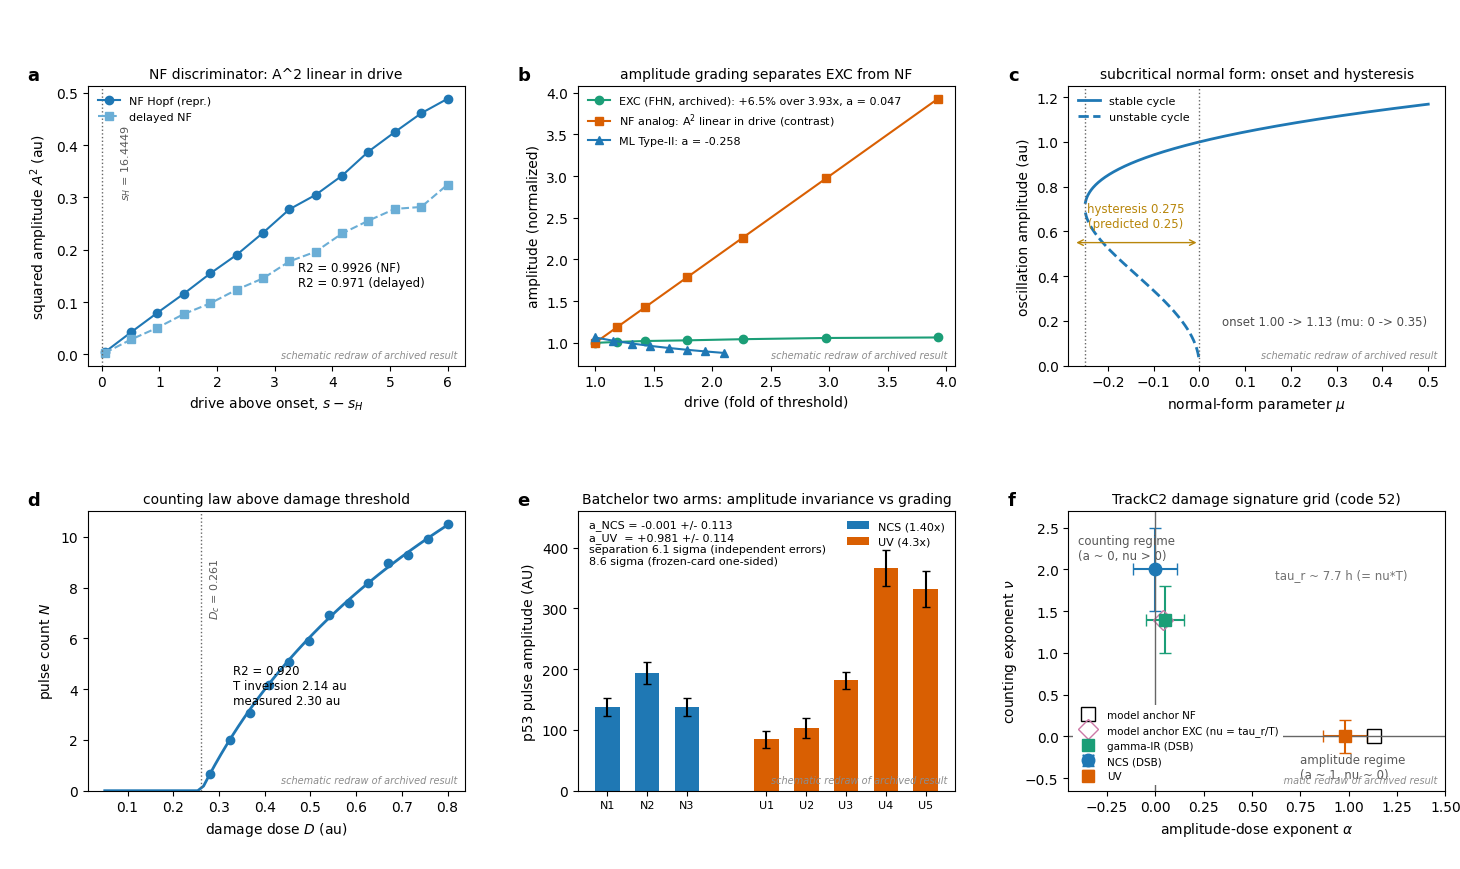
\includegraphics[width=\textwidth]{fig1_topology.png}
\caption{Class selection, numerics and evidence. \textbf{a}, NF discriminator: squared amplitude linear in drive above the Hopf point ($R^2=0.9926$; delayed variant $0.971$). \textbf{b}, Amplitude grading separates the classes: EXC holds $+6.5\%$ over a 3.9-fold drive ($\alpha=0.047$), NF gains $+360\%$, and the Morris--Lecar leaky-digital control sits an order of magnitude below NF ($\alpha=-0.258$). \textbf{c}, The subcritical escape hatch and how the remaining signatures close it (measured hysteresis $0.275$ versus normal-form $0.25$). \textbf{d}, The counting law above the damage threshold ($R^2=0.920$; slope inverts the period). \textbf{e}, The built-in two-arm control: digitised p53 pulse amplitudes after NCS (double-strand breaks, dose-invariant, 1.40$\times$ spread, non-monotone) and after UV (graded, 4.3$\times$ monotone), with the bootstrap separation annotated. \textbf{f}, The discrimination grid: measured $(\alpha,\nu)$ pairs for the two damage arms and the two model anchors, with the counting and amplitude regimes separated by an order of magnitude in $\alpha$. (Panels are schematic redraws of archived analysis results.)}
\label{fig:topology}
\end{figure}

\section{The published record decides the class}
\label{sec:evidence}

Batchelor \emph{et al.} \cite{Batchelor2011} provide a control built into a single study: the same protein in the same cell line (MCF7) shows excitable, fixed-amplitude, dose-counting pulses after double-strand breaks but a graded, non-excitable single pulse after UV. Digitising their Fig.~1G/H (colour-channel bar segmentation, visual axis calibration; extraction error $\pm14$--$30$ AU) gives NCS amplitudes ($100/200/400$ ng ml$^{-1}$) of $137.9/193.1/137.9$ AU, a non-monotone $1.40\times$ spread carrying no dose information, against UV amplitudes ($2/4/6/8/10$ J m$^{-2}$) of $84.8/103.3/181.5/366.3/331.5$ AU, monotone $4.3\times$ over the graded range. Durations concord (NCS exponent $-0.21$; UV exponent $+0.79$). Bootstrap resampling within the extraction-noise model ($\times20{,}000$) gives
\begin{equation}
\alpha_{\mathrm{NCS}}=-0.001\pm0.113\ (95\%\ \mathrm{CI}\ [-0.22,0.22]),
\qquad
\alpha_{\mathrm{UV}}=+0.981\pm0.114\ (95\%\ \mathrm{CI}\ [0.78,1.22]),
\label{eq:alphas}
\end{equation}
a separation of $6.1$ combined standard deviations under independent-error combination ($8.6$ under a single-sided denominator convention; no conclusion depends on the choice, as the class regions are an order of magnitude apart in $\alpha$). The NCS point estimate is not an independent measurement of flatness: the three concentrations are equally spaced in log dose and the two endpoint amplitudes are equal ($137.9$ AU each), so the ordinary least-squares slope vanishes by symmetry, and the informative quantity is the confidence half-width ($\pm0.11$), not the point value.

Placing all measured signatures on the discrimination grid (Table~\ref{tab:grid}, Fig.~\ref{fig:topology}f): both double-strand-break arms (NCS; $\gamma$-irradiation) land deep in the EXC region and the UV arm in the analogue region, co-varying with the source study's own excitability classification. The paper's verbatim anchors read: ``DSBs trigger a series of p53 pulses with fixed amplitude and duration, independent of the damage dose, whereas the number of pulses increases with higher damage,'' while the UV arm is a ``single pulse that increases in amplitude and duration in proportion to the UV dose'' \cite{Batchelor2011}.

\begin{table}[!htbp]
\centering
\caption{Measured $(\alpha,\nu)$ signatures on the discrimination grid. $\alpha$ from digitised dose series (bootstrap $\times20{,}000$); $\nu$ from the reported pulse-count statistics of \cite{Monke2017,Lahav2004}.}
\label{tab:grid}
\small
\begin{tabular}{@{}llll@{}}
\toprule
Data & $\alpha=\partial\ln A/\partial\ln D$ & $\nu=\partial N/\partial\ln D$ & Region \\
\midrule
NCS (DSB) & $-0.001\pm0.113$ & $2.0\pm0.5$ & EXC (counting) \\
$\gamma$-IR (DSB) & $0.05\pm0.10$ & $1.4\pm0.4$ & EXC (counting) \\
UV & $+0.981\pm0.114$ & $\approx0$ (single pulse) & analogue / NF-consistent \\
NF model anchor & $1.13$ & $\approx0$ & reference \\
EXC model anchor & $0.047$ & $\tau_r/T$ & reference \\
\bottomrule
\end{tabular}
\end{table}

The counting law has a regime boundary, and the literature locates it. Across twelve cell lines \cite{StewartOrnstein2017}, slow or failed DNA repair does not yield more pulses at fixed dose, as the naive counting picture predicts; it switches the encoder from the oscillatory regime to a sustained, graded regime (rank correlation between repair efficiency and oscillatory behaviour $\rho=+0.857$, one-sided $p=0.0068$ over the seven oscillatory lines). The counting law therefore holds inside the oscillatory regime, and repair failure is a change of language, not a louder signal.

\section{What the encoder can transmit: a channel census}
\label{sec:census}

\subsection{Protocol}

The class-level encoder is the EXC representative, a FitzHugh--Nagumo reduction with exponential damage repair,
\begin{equation}
\dot v=s\,(v-v^3/3-w)+\sigma\,\xi(t),
\qquad
\dot w=s\,\varepsilon\,(v+a-bw-I(t)),
\qquad
I(t)=I_0e^{-t/\tau_r},
\label{eq:fhn}
\end{equation}
with locked parameter set $s=20$, $\tau_r=20$, $a=0.7$, $b=0.8$, $\varepsilon=0.08$, $I_0=0.6$, $\sigma=0.06$. This is a universality-class representative, not a molecular model; conclusions carry the class-level reading. Six pulse statistics (first-pulse time $t_1$, period $T$, amplitude $A$, count $N$, width $w$, inter-pulse-interval dispersion $\mathrm{IPI}_{sd}$) are propagated onto the seven dynamical parameters: Monte Carlo ensembles ($M=400$ or $4000$ trajectories) give the statistic covariance $\Sigma_g$, finite-difference log-perturbations give the Jacobian, and the Fisher matrix is $F=J^{\mathsf T}\Sigma_g^{+}J$.

\subsection{Timing channels dominate; amplitude dies twice}

The parameter information distributes over the channels as: width $60.2\%$, count $18.2\%$, period $11.5\%$, first pulse $4.4\%$, interval dispersion $0.3\%$, amplitude $5.5\%$ (Fig.~\ref{fig:census}d). Timing-type channels thus carry the overwhelming share and amplitude almost none. We report the exact shares with an explicit calibration caveat: the decomposition depends on the representative's calibration. A mechanism-level recheck on the 23-parameter model shifts the nominal timing share to 45.1\% (amplitude 54.9\%), and across the defensible noise-calibration grid the timing share spans 0--91\%. The ordering is therefore calibration-dependent, and the share is reported as a representative-level result rather than an invariant.

The amplitude channel then dies a second, statistical death at the population layer. With per-cell gain dispersion $k_i\sim\mathrm{LogN}(0,\sigma_k)$, growing $\sigma_k$ from $0$ to $0.6$ drives the population $\mathrm{CV}(A)$ from $0.002$ to $0.639$, while $\mathrm{CV}(T)$ stays pinned at $0.016$ (Fig.~\ref{fig:census}f, inset): even the residual amplitude information is uncalibratable across cells, and timing survives both layers.

\subsection{Noise is an exact null direction of first-moment statistics}

The softest Fisher direction is the noise amplitude $\sigma$ itself (eigenvector weight $0.995$--$0.998$), with
\begin{equation}
\lambda_7/\lambda_1=4.7\times10^{-19}
\label{eq:null}
\end{equation}
at the reference configuration ($M=4000$, central differences). The ratio tracks the finite-difference resolution floor rather than a physical constant: it is $2.1\times10^{-18}$ at $M=400$ with a $2\%$ step, and at $M=4000$ with forward differences the seventh eigenvalue is negative ($-4.2\times10^{-13}$), so no exact null is resolved there (Fig.~\ref{fig:census}b,c). The content: mean-type pulse statistics are exactly blind to the fluctuation-generating noise; information about $\sigma$ lives exclusively in dispersion-type observables.

\subsection{Two dispersion signatures locate the stochastic sensing stage}

For any bare oscillator, $\mathrm{Var}(t_1)/\mathrm{Var}(T)$ is bounded at $0.03$--$0.12$. The measured value is $5.8$ (first-pulse dispersion $\pm240$ min versus interval dispersion $\pm100$ min \cite{Lahav2004,GevaZatorsky2006}), physically impossible for a bare oscillator. Adding one upstream exponential stochastic delay $\tau_d\sim\mathrm{Exp}(\mu_d)$, standing in for the ATM sensing stage, flips the ratio monotonically, and at $\mu_d\approx T$ reproduces $5.7\approx5.8$ (Fig.~\ref{fig:census}e). Independently, slow parameter heterogeneity inflates population $\mathrm{CV}(T)$ while pinning intra-cellular $\mathrm{IPI}_{\mathrm{CV}}$ at $0.083$, whereas fast white noise moves both together; the measured $\mathrm{IPI}_{\mathrm{CV}}=0.30$ is reachable only by fast intra-cellular stochasticity. The two dispersion axes thereby separate fluctuation sources by time colour, refining rather than contradicting the slow-noise reading of \cite{GevaZatorsky2006}.

\subsection{The digital limit, verified}

With counting law $N(D)=\rho\ln(D_0(D)/D_c)$, per-dose counts Poisson, amplitude observable $\bar y\sim\mathcal{N}(sA,\sigma^2)$ at $15\%$ noise, and parameter vector $(\ln D_c,\ln\rho,\ln A,\ln s)$: the counting-only Fisher spectrum is $[26935,\,1898,\,0,\,0]$, exactly two nonzero structural directions; adding the amplitude observable adds exactly one direction (the product $sA$), and the zero-direction eigenvector $(0,0,1,-1)/\sqrt2$ coincides with the scale-degeneracy orbit tangent at cosine $1.000000$. Monte Carlo estimation against the Cram\'er--Rao bound gives ratios $1.24$ ($\ln\rho$), $1.36$ ($\ln D_c$) and $0.95$ for the estimable combination $\ln(sA)$; fixing the scale $s$ at a wrong value leaves the likelihood invariant under the compensation $\hat A=sA/s$. The scale direction is not merely small, it is structurally zero, and the structural parameters exhaust their information bound.

\subsection{The counting channel is near-lossless}

Over a four-fold dose range, the mutual information between dose and pulse count is
\begin{equation}
I(D;N)=3.07\ /\ 3.17\ \text{bits}\ \ (96.8\%),
\label{eq:capacity}
\end{equation}
with the counting law $N\approx10.5\ln I_0+c$ linear throughout (Fig.~\ref{fig:census}f). The digital channel is not a lossy compromise; it attains essentially its full efficiency ceiling.

\begin{figure}[p]
\centering
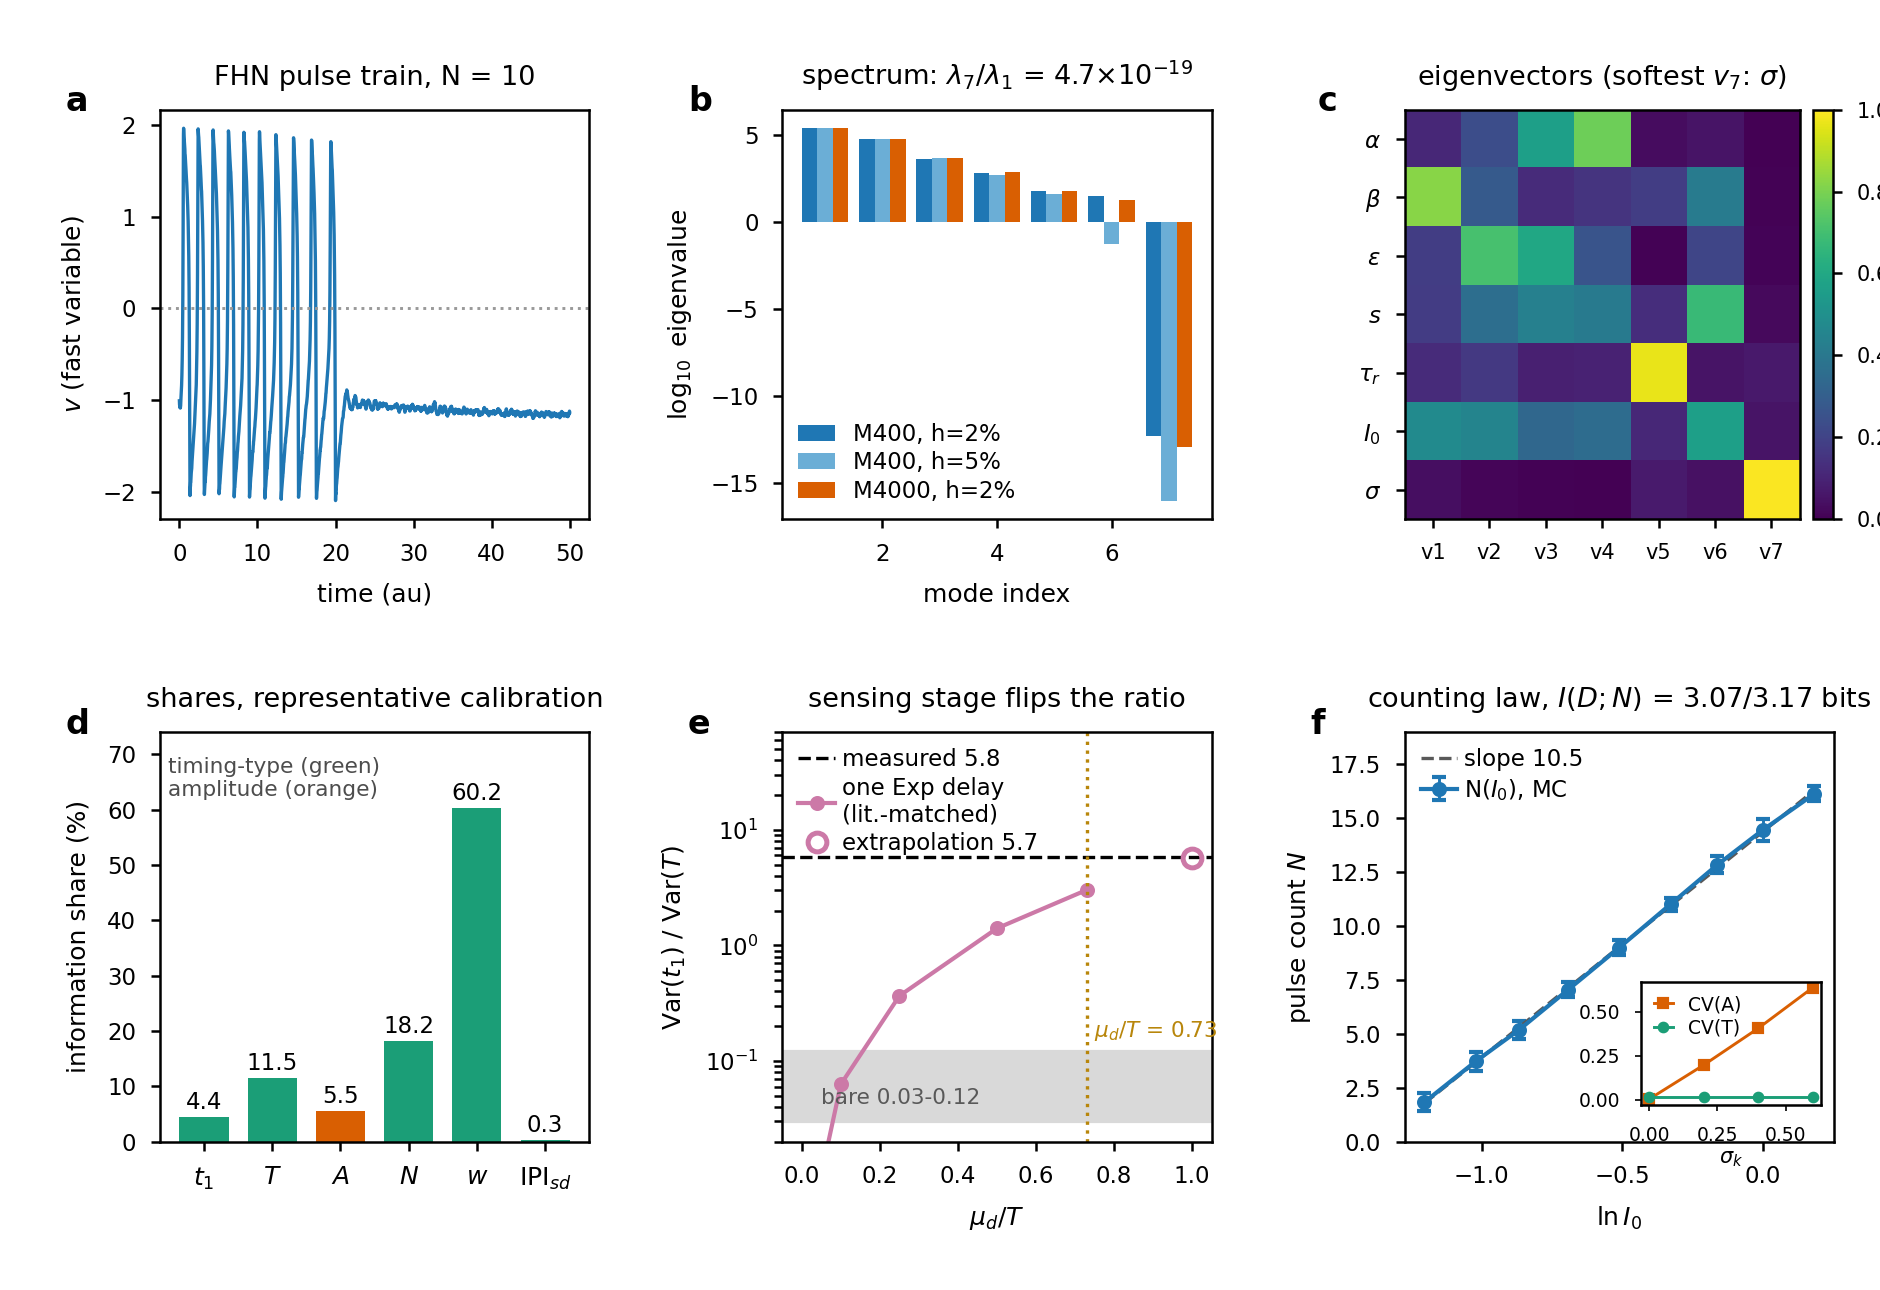
\includegraphics[width=\textwidth]{fig2_census.png}
\caption{The channel census of the excitable encoder. \textbf{a}, Reference pulse train of the FitzHugh--Nagumo representative under Eq.~\eqref{eq:fhn}. \textbf{b}, Fisher spectrum across three numerical configurations; the seventh direction sits at the resolution floor in every configuration ($\lambda_7/\lambda_1=4.7\times10^{-19}$ at the reference configuration). \textbf{c}, Eigenvector composition; the softest direction is the noise amplitude $\sigma$ (weight $0.996$). \textbf{d}, Channel shares of parameter information: timing-type channels $94.5\%$, amplitude $5.5\%$ (representative calibration; the share is calibration-bounded and the ordering is not claimed as invariant). \textbf{e}, First-pulse dispersion ratio $\mathrm{Var}(t_1)/\mathrm{Var}(T)$ under one upstream exponential sensing delay (literature-matched calibration): bare oscillators sit at $0.03$--$0.12$ (shaded band); the measured $5.8$ (dashed) is reached at $\mu_d\approx T$ (open marker: quadratic extrapolation of the calibrated segment, registered in the Discussion). \textbf{f}, The counting law $N\approx10.5\ln I_0+c$ with $I(D;N)=3.07/3.17$ bits; inset, the gain-dispersion kill: population $\mathrm{CV}(A)$ rises with gain dispersion while $\mathrm{CV}(T)$ stays pinned.}
\label{fig:census}
\end{figure}

\section{The molecular origin of the 5.5-hour clock}
\label{sec:molecular}

The timing observables decompose onto the kinetic constants of the reconstructed 23-parameter mechanism model (\cite{Monke2017} calibration with the 2025 revision \cite{Venkatachalapathy2025}; modelling lineage \cite{Monk2003,BarOr2000,Ciliberto2005,Chickarmane2007,NovakTyson2008}). Entering constants are classified as measured, distribution-bounded, or registered gaps. Of the four Wip1-arm constants, $T_W$ is a universal biophysical candidate, $d_W$ is bounded by a threefold spread across sources, and $T_w$ (mRNA production) and $P$ (Wip1 dephosphorylation of ATM$^*$) are registered gaps; no timing conclusion rests on a free fitting parameter introduced by this work.

\paragraph{Period.} Linearising the six-species model at its operating point gives a dominant Jacobian eigenvalue $0.627+1.057i$, that is, $T=2\pi/1.057=5.95$ h against the simulated $5.48$ h (8.5\% deviation, registered; the linear prediction inherits the model's own width bias). Phase-share attribution over the cycle: p53 30\%, ATM* 24\%, mdm2 mRNA 18\%, wip1 mRNA 15\%, Wip1 protein 10\%, Mdm2 protein 2\% (Fig.~\ref{fig:molecular}c). The period-from-constants direction has prior art in simplified cores \cite{Monk2003,Wang2019,Belgacem2026}; the contribution here is the complete six-species attribution.

\paragraph{Interval and first-pulse delay.} Phase-space decomposition gives the interpulse interval as $1.70$ h (phase estimate) against the measured $2.0\pm0.5$ h, and the Wip1-arm delay, the model's proxy for the first-pulse delay, as $1.13$ h against the $1.25$ h anchor (Fig.~\ref{fig:molecular}a,b). Both are registered as consistency closures rather than independent predictions, because the model-calibrated constants in the sums were themselves anchored on the same measured bands; the non-circular content is the absence of inconsistency at the stated precision.

\paragraph{Pulse width.} Simulated FWHM $2.78$ h, decomposing into a $0.79$ h rise-to-ATM$^*$-off segment plus a $1.99$ h collapse tail dominated by Mdm2 recovery, dose-independent (CV $0.055$ across the dose grid). The segment sum equals the FWHM by construction, so the content of the decomposition is the attribution, not the arithmetic. A literature-internal conflict is registered: Wip1 at 85\% widens pulses by $+30\%$ and at 70\% locks the model into the sustained state, whereas \cite{Monke2017} report approximate width invariance; the conflict between \cite{Batchelor2011} and \cite{Monke2017} on this point is recorded, not resolved.

\paragraph{Independent closed-form cross-validation.} Belgacem's logistic-substitution DDE model of the p53--Mdm2 core \cite{Belgacem2026} was reproduced independently: his closed-form period reproduces under his calibration ($T=5.642$ h), our independent DDE integration of his equations gives $5.646$ h (0.07\% apart), and a state-consistency constraint emerges (Fig.~\ref{fig:closedform}): his basal-state half-lives with the measured 2 h delay yield $T=8.40$ h, failing against experiment, while the stressed-state parameter set yields $T=5.60$ h, a three-way agreement between the measured $5.5$ h, his closed form, and our six-species simulation $5.48$ h. Oscillatory-regime parameters must be read as stressed-state quantities, not basal-state ones.

\paragraph{Registered boundaries.} (i) The linear-eigenvalue period overshoots the simulation by 8.5\%, and the model width ($2.78$ h) sits below the archived 3.5 h band; both directions are consistent with the mechanism core running slightly fast and narrow under the nominal calibration. (ii) The counting-law threshold $D_c$ differs between the digitised archive scale (0.261 Gy) and the mechanism-level scale (0.99 Gy), a factor $3.8$. The discrepancy is conducted entirely by the assumed conversion of 35 DSB per Gy; the experimental literature bounds plausible conversions at 20--40 DSB per Gy \cite{Rothkamm2003}, and closing the tension would require $\sim$9, far outside the band. The tension is therefore established as real, and the counting-law slope of Lemma 3 is quoted on the digitised scale only.

\begin{figure}[p]
\centering
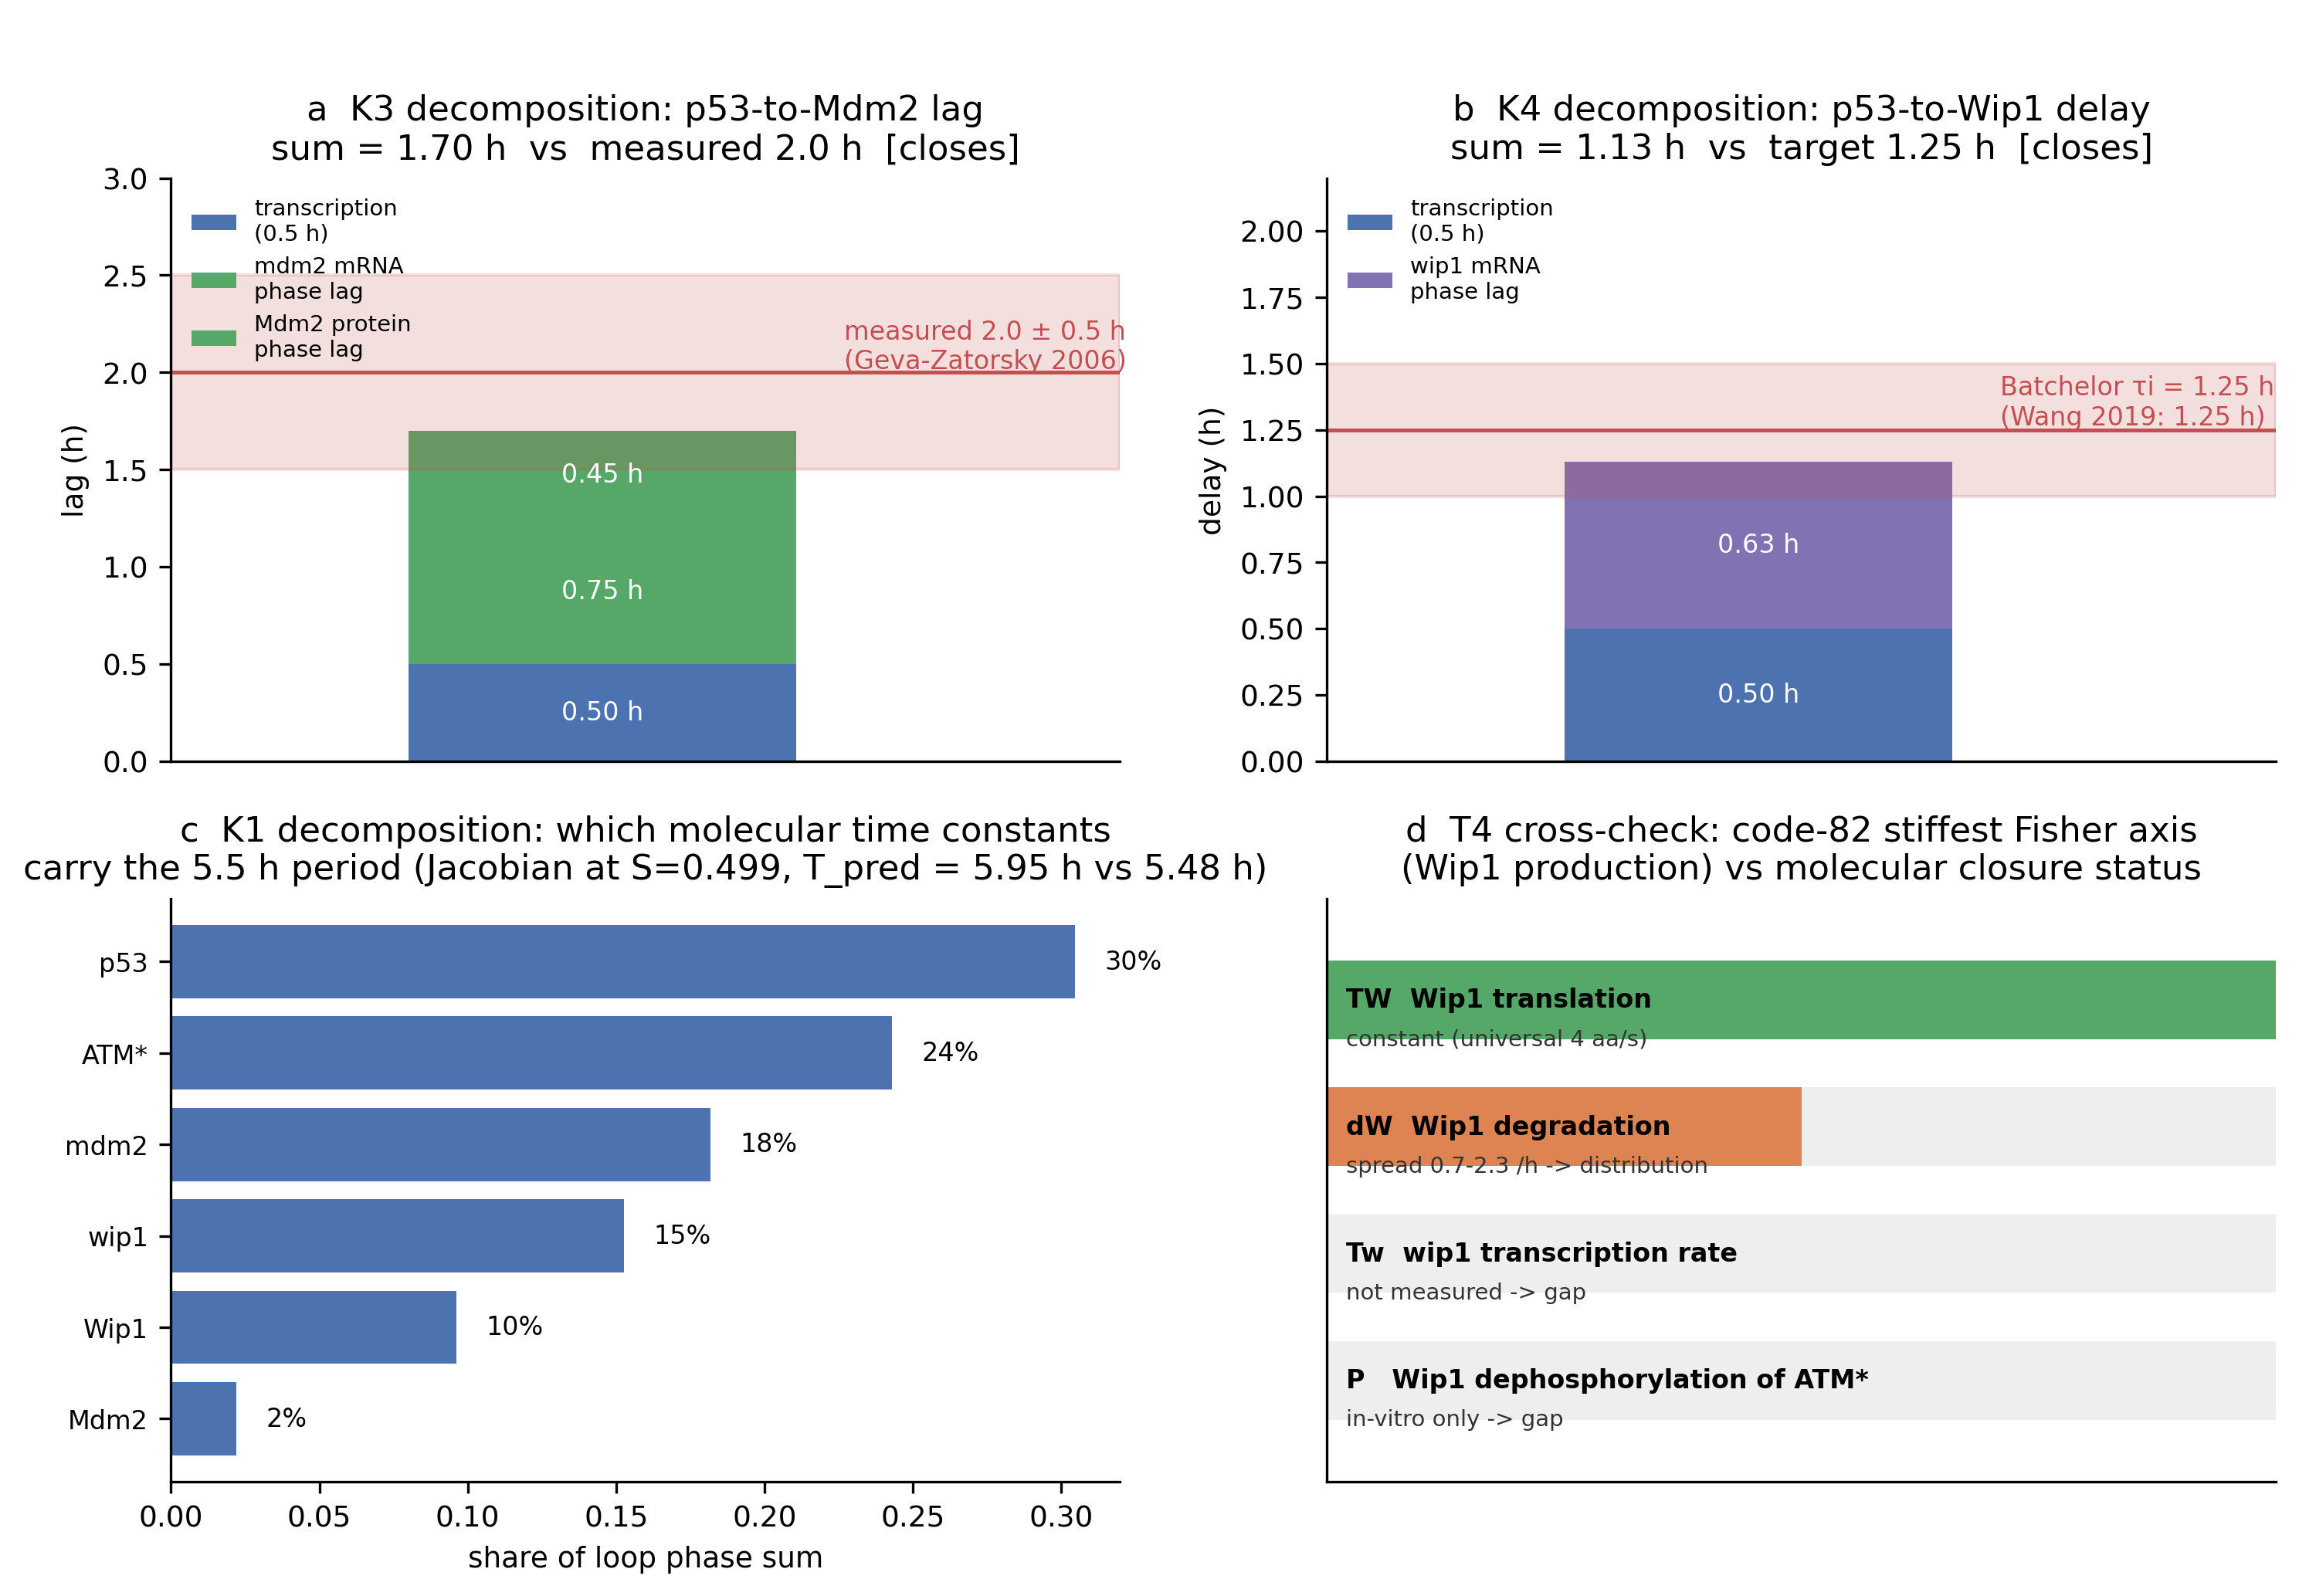
\includegraphics[width=\textwidth]{fig3_molecular.png}
\caption{Molecular decomposition of the timing constants. \textbf{a}, Interpulse-interval decomposition ($1.70$ h phase estimate against the measured $2.0\pm0.5$ h band). \textbf{b}, First-pulse-delay decomposition ($1.13$ h against the $1.25$ h anchor). \textbf{c}, Phase-share attribution of the $5.5$ h period across the six molecular species (Jacobian prediction $5.95$ h versus simulation $5.48$ h). \textbf{d}, Closure status of the Wip1 arm constants, with the stiffest Fisher axis (Wip1 production) marked: one measured constant, one distribution-bounded, two registered gaps.}
\label{fig:molecular}
\end{figure}

\begin{figure}[p]
\centering
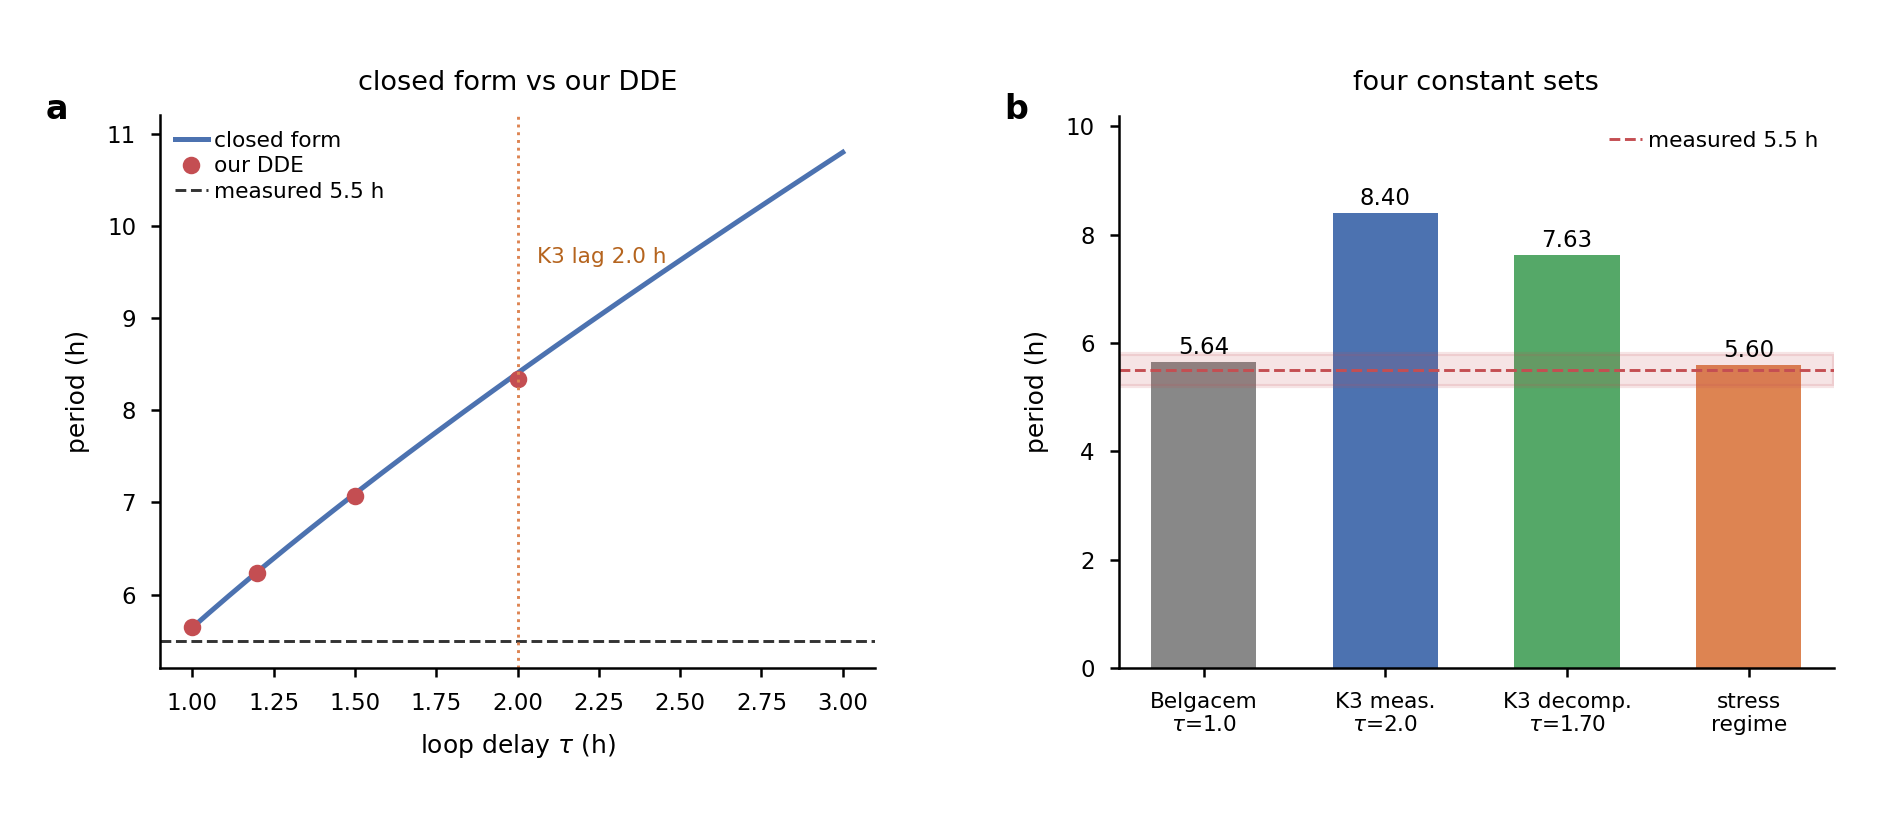
\includegraphics[width=\textwidth]{fig4_closedform.png}
\caption{Independent closed-form cross-validation. \textbf{a}, Belgacem's closed-form period as a function of loop delay (line), overlaid with our independent Python DDE integration of his equations (points); the measured 5.5 h period and our six-species simulation 5.48 h sit at the dashed line. \textbf{b}, The same closed form evaluated under four constant sets: Belgacem's own calibration ($5.64$ h) and the stressed-state set (fast p53 turnover, $5.60$ h) land on the measured period, while the basal-state half-lives fail, at $8.40$ h with the measured $2.0$ h delay and at $7.63$ h with the decomposed $1.70$ h delay.}
\label{fig:closedform}
\end{figure}

\section{The decisive experiment that has never been done}
\label{sec:hysteresis}

The theorem's strongest attack surface is the subcritical escape hatch (Section~\ref{sec:theorem}), and its closure requires the second signature: hysteresis width. No published p53 dose series is a two-way scan; all are one-way. The protocol is therefore specified here with frozen decision criteria. System: MCF7 p53-CFP/Mdm2-YFP single cells \cite{Lahav2004}, live-cell time-lapse, 20 min frames, $\ge16$ h. Dose ladder: NCS $25\to50\to100\to200\to400\to200\to100\to50\to25$ ng ml$^{-1}$, dwelling 4--6 h per step, or an equivalent stepped $\gamma$-irradiation design, with a one-way ascending control arm on the same cell population. Readout: onset is the first-pulse dose on the up-scan, extinction the last-pulse dose on the down-scan, width $w=|\mathrm{onset}-\mathrm{extinction}|$/active window. Decision: $w<5\%$ is EXC-consistent (the prediction); $w\ge5\%$ forces reclassification to the subcritical column, downgrading ``excluding pure negative feedback'' to ``excluding supercritical NF''. Power: at $\le15\%$ amplitude precision, $\alpha$ is estimated to $\approx0.075$, below the inter-class gap of $0.2$; $n=30$--$50$ cells per arm suffice. Registered risks: NCS is an irreversible damaging agent, so descending-limb extinction may be confounded by damage accumulation, countered by pulsed dosing with washout; the irradiation arm confounds cumulative with instantaneous dose, and the two arms serve as mutual controls.

\section{Discussion}

The question ``why does p53 count?'' has a two-part answer. First, it has no choice: the amplitude channel of an excitable encoder is closed by geometry, and the published two-arm record assigns the DSB response to that class at $6.1\sigma$. Second, counting is not a poor substitute: the count channel attains 96.8\% of its information ceiling, its statistics are blind to the fluctuation noise to numerical resolution ($\lambda_7/\lambda_1=4.7\times10^{-19}$ at the reference configuration), and its timing constants decompose onto measured molecular rates. The encoder's design logic reads as economy, not accident.

The regime boundary is as informative as the rule. The same protein switches classes with damage type (counting after double-strand breaks, graded after UV \cite{Batchelor2011}), and repair failure switches oscillatory cell lines into a sustained regime \cite{StewartOrnstein2017}: the counting law is a property of the oscillatory regime, and the cell possesses both languages.

Limitations are explicit. The separation theorem is proven for the two generic classes with the stated premises (two-time-scale structure, fold destabilisation, drive entering the slow equation); exotic architectures outside the classes are out of scope. The channel census uses a universality-class representative; both the shares and the ordering are calibration-bounded (45.1\% versus 54.9\% timing-to-amplitude at the 23-parameter mechanism level), so the census is reported at the representative level. The dispersion-ratio inversion quotes a quadratic extrapolation from the calibrated segment rather than a simulated point. The digitised evidence carries registered extraction error bands, and the $D_c$ scale tension between digitised and mechanism-level calibrations is established, not resolved. The hysteresis experiment is proposed, not performed.

\section{Methods}
\label{sec:methods}

\subsection{Model classes and numerics}

NF representatives (three-ODE Goodwin-type and delayed variants) and the EXC representative (FitzHugh--Nagumo with slow drive, Eq.~\eqref{eq:fhn}) were integrated with synchronous explicit schemes; onset branches were obtained by continuation. Hopf-onset scaling was verified by least squares of $A^2$ against $s-s_H$ ($R^2=0.9926$; delayed variant $0.971$). The subcritical normal form $\dot z=(\mu+i)z+|z|^2z-|z|^4z$ supplied the hysteresis control. The Morris--Lecar Type-II model served as the fast-equation-drive control. The counting law \eqref{eq:counting} was fit to simulated pulse counts ($R^2=0.920$).

\subsection{Data and digitisation}

Published dose-response statistics were taken from \cite{Lahav2004,GevaZatorsky2006,Batchelor2011,Monke2017,Loewer2013,StewartOrnstein2017,Loewer2010}. Figure-level digitisation of \cite{Batchelor2011} Fig.~1G/H used colour-channel bar segmentation with visual axis calibration; extraction error bands ($\pm14$--$30$ AU) were registered and propagated by bootstrap ($\times20{,}000$) into the $\alpha$ estimates of Eq.~\eqref{eq:alphas}.

\subsection{Fisher propagation and information estimates}

Monte Carlo ensembles ($M=400$ or $4000$ trajectories) of Eq.~\eqref{eq:fhn} gave the covariance of six pulse statistics; per-parameter log-perturbations ($\pm2\%$/$\pm5\%$ double runs; $\pm8\%$ for the discrete count channel) gave the Jacobian by finite differences; $F=J^{\mathsf T}\Sigma_g^{+}J$ with pseudoinverse truncation $10^{-12}$. Three numerical configurations (central/forward differences) were run for all spectral claims. Mutual information used the binned estimator with the registered caveat that trends are reliable while absolute values are mildly biased. Quality control: two internal implementation errors (a pulse-width extraction off-by-one; a semi-implicit integrator mis-step) were caught by their physically impossible signatures, repaired, and independently rerun; no reported value moved.

\subsection{Molecular decomposition and cross-validation}

The 23-parameter mechanism model of \cite{Monke2017,Venkatachalapathy2025} was linearised at its operating point for the period and phase shares; interval and delay sums were decomposed by phase-space bookkeeping; pulse width was measured as FWHM over the dose grid. The closed-form oscillator of \cite{Belgacem2026} was reproduced and independently integrated as a DDE. All scripts are deterministic under fixed seeds. The digitised Batchelor Fig.~1G/H extraction is shipped with the repository (\texttt{data\_external/batchelor2011/digitized\_Fig1GH.json}) and is the direct input of code52; re-running it reproduces the $\alpha$ estimates of Eq.~\eqref{eq:alphas} bit-for-bit.

\subsection{Reproducibility}

Analysis scripts (codes 13, 50--52, 81, 82, 89--93, and the bifurcation-and-discrimination suite of cell line 1, all archived in the same repository) and extracted tables are available at \url{github.com/lihuanlz/p53-pulse-encoder}, archived at Zenodo (doi:10.5281/zenodo.23402854; umbrella edition: doi:10.5281/zenodo.23008824).

\section*{Data and code availability}

No new experimental data were generated. All analysis scripts and digitised tables are available at \url{github.com/lihuanlz/p53-pulse-encoder}, archived at Zenodo (doi:10.5281/zenodo.23402854; umbrella edition: doi:10.5281/zenodo.23008824).

\section*{Acknowledgements}

This work re-analyses public single-cell data and published models. We thank G.~Lahav and colleagues, E.~Batchelor and colleagues, G.~M\"onke, A.~Loewer and colleagues, J.~Stewart-Ornstein, and I.~Belgacem for the measurements, models and closed forms on which the analysis rests.

\section*{Author contributions}

H.L.\ conceived the study, proved the theorem-level statements, wrote and validated the analysis code, performed the analysis, and wrote the paper.

\section*{Competing interests}

The author declares no competing interests.

\begin{thebibliography}{99}
\small

\bibitem{Lahav2004}
Lahav, G. et al. Dynamics of the p53--Mdm2 feedback loop in individual cells. \emph{Nat. Genet.} \textbf{36}, 147--150 (2004).

\bibitem{GevaZatorsky2006}
Geva-Zatorsky, N. et al. Oscillations and variability in the p53 system. \emph{Mol. Syst. Biol.} \textbf{2}, 2006.0033 (2006).

\bibitem{Batchelor2008}
Batchelor, E., Mock, C.~S., Bhan, I., Loewer, A. \& Lahav, G. Recurrent initiation: a mechanism for triggering p53 pulses in response to DNA damage. \emph{Mol. Cell} \textbf{30}, 277--289 (2008).

\bibitem{Batchelor2011}
Batchelor, E., Loewer, A., Mock, C. \& Lahav, G. Stimulus-dependent dynamics of p53 in single cells. \emph{Mol. Syst. Biol.} \textbf{7}, 488 (2011).

\bibitem{Loewer2013}
Loewer, A., Karanam, K., Mock, C. \& Lahav, G. The p53 response in single cells is linearly correlated to the number of DNA breaks without a distinct threshold. \emph{BMC Biol.} \textbf{11}, 114 (2013).

\bibitem{Monke2017}
M\"onke, G. et al. Excitability in the p53 network mediates robust signaling with tunable activation thresholds in single cells. \emph{Sci. Rep.} \textbf{7}, 46571 (2017).

\bibitem{Venkatachalapathy2025}
Venkatachalapathy, H., Dallon, S., Yang, Z., Azarin, S.~M., Sarkar, C.~A. \& Batchelor, E. Pulsed stimuli enable p53 phase resetting to synchronize single cells and modulate cell fate. \emph{Mol. Syst. Biol.} \textbf{21}, 390--412 (2025).

\bibitem{StewartOrnstein2017}
Stewart-Ornstein, J. \& Lahav, G. p53 dynamics in response to DNA damage vary across cell lines and are shaped by efficiency of DNA repair and activity of the kinase ATM. \emph{Sci. Signal.} \textbf{10}, eaah6671 (2017).

\bibitem{BarOr2000}
Bar-Or, R.~L. et al. Generation of oscillations by the p53--Mdm2 feedback loop: a theoretical and experimental study. \emph{Proc. Natl Acad. Sci. USA} \textbf{97}, 11250--11255 (2000).

\bibitem{Monk2003}
Monk, N.~A.~M. Oscillatory expression of Hes1, p53, and NF-$\kappa$B driven by transcriptional time delays. \emph{Curr. Biol.} \textbf{13}, 1409--1413 (2003).

\bibitem{Ciliberto2005}
Ciliberto, A., Nov\'ak, B. \& Tyson, J.~J. Steady states and oscillations in the p53/Mdm2 network. \emph{Cell Cycle} \textbf{4}, 488--493 (2005).

\bibitem{Chickarmane2007}
Chickarmane, V., Ray, A., Sauro, H.~M. \& Nadim, A. A model for p53 dynamics triggered by DNA damage. \emph{SIAM J. Appl. Dyn. Syst.} \textbf{6}, 61--78 (2007).

\bibitem{NovakTyson2008}
Nov\'ak, B. \& Tyson, J.~J. Design principles of biochemical oscillators. \emph{Nat. Rev. Mol. Cell Biol.} \textbf{9}, 981--991 (2008).

\bibitem{Wang2019}
Wang, C., Liu, H. \& Zhou, J. Contribution of time delays to p53 oscillation in DNA damage response. \emph{IET Syst. Biol.} \textbf{13}, 180--185 (2019).

\bibitem{Belgacem2026}
Belgacem, I. Sustained limit cycles in the logistic two-gene genetic oscillator: a delay-driven Hopf bifurcation. Preprint at arXiv \url{https://arxiv.org/abs/2605.23722} (2026).

\bibitem{Soule2003}
Soul\'e, C. Graphic requirements for multistationarity. \emph{ComPlexUs} \textbf{1}, 123--133 (2003).

\bibitem{Gouze1998}
Gouz\'e, J.-L. Positive and negative circuits in dynamical systems. \emph{J. Biol. Syst.} \textbf{6}, 11--15 (1998).

\bibitem{Rothkamm2003}
Rothkamm, K. \& L\"obrich, M. Evidence for a lack of DNA double-strand break repair in human cells exposed to very low X-ray doses. \emph{Proc. Natl Acad. Sci. USA} \textbf{100}, 5057--5062 (2003).

\bibitem{Loewer2010}
Loewer, A., Batchelor, E., Gaglia, G. \& Lahav, G. Basal dynamics of p53 reveal transcriptionally attenuated pulses in cycling cells. \emph{Cell} \textbf{142}, 89--100 (2010).

\end{thebibliography}

\end{document}
